%%%%%%%%%%%%%%%%%%%%%%%%%%%
%%  Componenti del back end
%%%%%%%%%%%%%%%%%%%%%%%%%%%



\subsection{\nogloxy{swedesigner::server}}
\label{\nogloxy{swedesigner::server}}
\subsubsection{Informazioni generali}
\begin{figure}[H]
	\makebox[\textwidth][c]{
	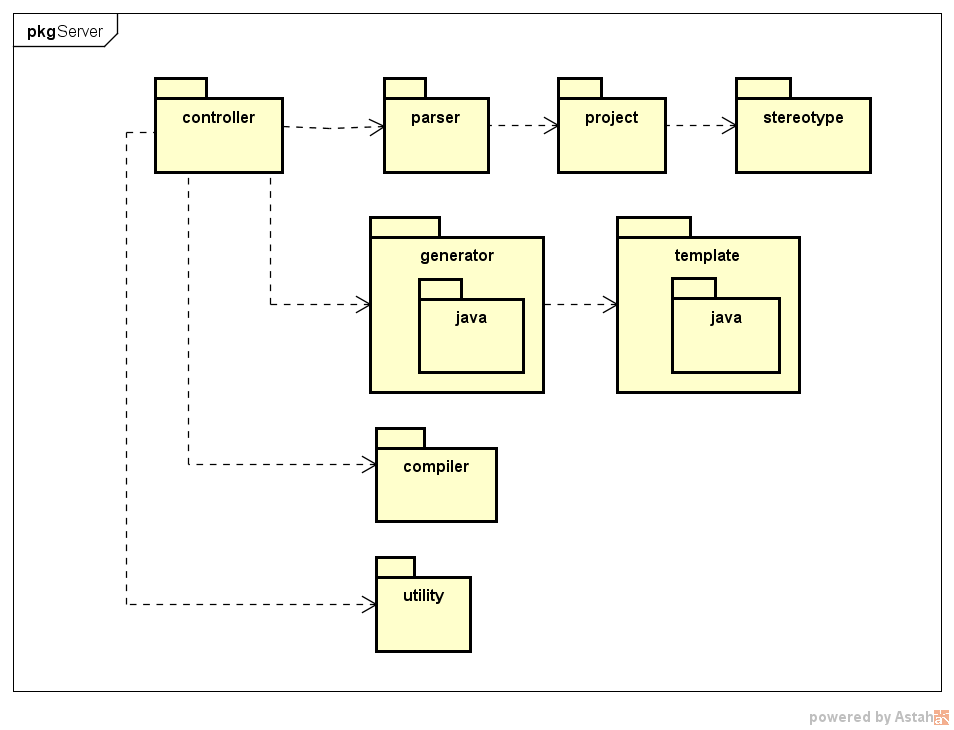
\includegraphics[width=1\textwidth]{img/server_pkg}}
	\caption{Diagramma package server}
\end{figure}
\begin{itemize}
\item \textbf{Descrizione}\\
Questo package contiene le componenti del server, scritte in Java.
\item \textbf{Padre}: \hyperref[\nogloxy{swedesigner}]{\nogloxy{\texttt{swedesigner}}}
\item \textbf{Package contenuti}:
\begin{itemize}
\item \hyperref[\nogloxy{swedesigner::server::compiler}]{\nogloxy{\texttt{compiler}}}\\
Questo package contiene le classi adibite alla compilazione del codice sorgente in codice eseguibile (nel linguaggio target specifico). È stata prevista la possibilità di ampliare questo package inserendo al suo interno ulteriori package. All'interno di questo package è presente unicamente il package \texttt{java}.
\item \hyperref[\nogloxy{swedesigner::server::controller}]{\nogloxy{\texttt{controller}}}\\
Questo package contiene i vari controller che implementano il pattern Front Controller fornito dal framework \emph{Spring}. Ogni controller dovrebbe occuparsi di gestire una richiesta e di rispondere opportunamente ad essa, attraverso l'interfaccia REST definita.
\item \hyperref[\nogloxy{swedesigner::server::generator}]{\nogloxy{\texttt{generator}}}\\
Questo package contiene le classi adibite alla trasformazione dal diagramma (rappresentato in oggetti Java derivati da oggetti JSON) a codice sorgente, nel linguaggio target specifico. È stata prevista la possibilità di ampliare questo package inserendo al suo interno ulteriori package. All'interno di questo package è presente unicamente il package \texttt{java}.
\item \hyperref[\nogloxy{swedesigner::server::parser}]{\nogloxy{\texttt{parser}}}\\
Questo package presenta le classi utili all'attività di parsing dei dati ricevuti dai client.
\item \hyperref[\nogloxy{swedesigner::server::project}]{\nogloxy{\texttt{project}}}\\
Questo package contiene al suo interno le classi utili a rappresentare un progetto UML. Il package parser necessita di questo package per poter dare in output un programma rappresentato in memoria come oggetti Java. Per chiarezza e per evitare l'uso di keyword riservate dal linguaggio Java, all'inizio del nome di queste classi è inserito il prefisso \texttt{Parsed} (e.g. \texttt{ParsedClass}).
\item \hyperref[\nogloxy{swedesigner::server::stereotype}]{\nogloxy{\texttt{stereotype}}}\\
Questo package offre le classi che descrivono ciò che caratterizza un particolare stereotipo. Queste classi derivano tutte da una classe base chiamata \texttt{Stereotype}. Le classi che definiscono come deve variare ogni stereotipo sono contraddistinte dal suffisso \texttt{Stereotype} (e.g. \texttt{BoardStereotype}). Si noti che tra queste classi non sono presenti dei legami, in quanto sono necessarie alla generazione del codice. La struttura degli stereotipi assegnabili ad ogni classe e le loro relazioni saranno definite successivamente nella \emph{Definizione di Prodotto}.
\item \hyperref[\nogloxy{swedesigner::server::template}]{\nogloxy{\texttt{template}}}\\
Questo package contiene le classi necessarie a trasformare l'oggetto che rappresenta il programma in una stringa di testo che rappresenta il codice sorgente tramite un sistema a template, il quale definirà tramite dei file di testo la struttura di ogni componente del programma; per facilitare questo compito sarà usata la libreria \stringtemplate{}. Similarmente al package \texttt{Generator} si è prevista la possibilità di implementare un sistema di template per ogni linguaggio, implementando diversamente l'interfaccia della classe Template e definendo un nuovo package (e.g. \texttt{Java}).
\item \hyperref[\nogloxy{swedesigner::server::utility}]{\nogloxy{\texttt{utility}}}\\
Questo package contiene le componenti secondarie necessarie al server, indipendentemente dal linguaggio target dell'applicazione.
\end{itemize}
\end{itemize}
\subsubsection{Classi}
\subsubsubsection{\nogloxy{swedesigner::server::Application}}
\label{\nogloxy{swedesigner::server::Application}}
\begin{itemize}
\item \textbf{Descrizione}\\
Classe principale che consente l'avvio dell'applicazione spring.
\item \textbf{Utilizzo}\\
La classe viene utilizzata per avviare l'applicazione spring
\end{itemize}
\subsection{\nogloxy{swedesigner::server::compiler}}
\label{\nogloxy{swedesigner::server::compiler}}
\subsubsection{Informazioni generali}
\begin{figure}[H]
	\makebox[\textwidth][c]{
	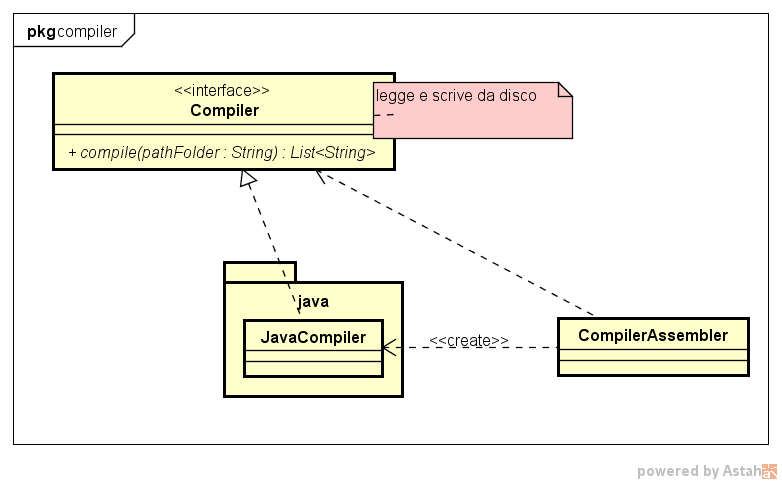
\includegraphics[width=1\textwidth]{img/server_compiler}}
	\caption{Diagramma package server::compiler}
\end{figure}
\begin{itemize}
\item \textbf{Descrizione}\\
Questo package contiene le classi adibite alla compilazione del codice sorgente in codice eseguibile (nel linguaggio target specifico). È stata prevista la possibilità di ampliare questo package inserendo al suo interno ulteriori package. All'interno di questo package è presente unicamente il package \texttt{java}.
\item \textbf{Padre}: \hyperref[\nogloxy{swedesigner::server}]{\nogloxy{\texttt{server}}}
\item \textbf{Package contenuti}:
\begin{itemize}
\item \hyperref[\nogloxy{swedesigner::server::compiler::java}]{\nogloxy{\texttt{java}}}\\
Questo package offre un'implementazione dell'interfaccia \texttt{Compiler} appartenente al package superiore. Possono essere aggiunti simili package per permettere la generazione in altri linguaggi.
\end{itemize}
\end{itemize}
\subsubsection{Classi}
\subsubsubsection{\nogloxy{swedesigner::server::compiler::Compiler}}
\label{\nogloxy{swedesigner::server::compiler::Compiler}}
\begin{itemize}
\item \textbf{Descrizione}\\
questa interfaccia si occupa di fornire un oggetto compiler generico a chi lo richiede in modo da poter rendere entensibile il sistema aggiungendo un'implementazione concreta del compiler del linguaggio target desiderato.
\item \textbf{Utilizzo}\\
\textt{RequestHandlerController} ha una dipendenza verso \texttt{Compiler} in quanto chiederà a \textt{CompilerAssembler} una implementazione concreta di un \textt{Compiler} in base al linguaggio target. Il pattern realizzato con questa classe è una \emph{dependency injection}.
\item \textbf{Relazioni con altre classi}:
\begin{itemize}
\item \textit{IN} \hyperref[\nogloxy{swedesigner::server::compiler::java::JavaCompiler}]{\nogloxy{\texttt{JavaCompiler}}}\\
questa classe è una implementazione di \texttt{Compiler} che permette di creare un jar dal codice sorgente Java.
\item \textit{IN} \hyperref[\nogloxy{swedesigner::server::controller::RequestHandlerController}]{\nogloxy{\texttt{RequestHandlerController}}}\\
questa classe si occupa di ricevere le richieste REST provenienti dal client.
\end{itemize}
\end{itemize}
\subsection{\nogloxy{swedesigner::server::compiler::java}}
\label{\nogloxy{swedesigner::server::compiler::java}}
\subsubsection{Informazioni generali}
\begin{itemize}
\item \textbf{Descrizione}\\
Questo package offre un'implementazione dell'interfaccia \texttt{Compiler} appartenente al package superiore. Possono essere aggiunti simili package per permettere la generazione in altri linguaggi.
\item \textbf{Padre}: \hyperref[\nogloxy{swedesigner::server::compiler}]{\nogloxy{\texttt{compiler}}}
\end{itemize}
\subsubsection{Classi}
\subsubsubsection{\nogloxy{swedesigner::server::compiler::java::JavaCompiler}}
\label{\nogloxy{swedesigner::server::compiler::java::JavaCompiler}}
\begin{itemize}
\item \textbf{Descrizione}\\
questa classe è una implementazione di \texttt{Compiler} che permette di creare un jar dal codice sorgente Java.
\item \textbf{Utilizzo}\\
viene utilizzata da \texttt{CompilerAssembler} che ritorna un' istanza di essa quando richiesto.
\item \textbf{Relazioni con altre classi}:
\begin{itemize}
\item \textit{OUT} \hyperref[\nogloxy{swedesigner::server::compiler::Compiler}]{\nogloxy{\texttt{Compiler}}}\\
questa interfaccia si occupa di fornire un oggetto compiler generico a chi lo richiede in modo da poter rendere entensibile il sistema aggiungendo un'implementazione concreta del compiler del linguaggio target desiderato.
\end{itemize}
\end{itemize}
\subsection{\nogloxy{swedesigner::server::controller}}
\label{\nogloxy{swedesigner::server::controller}}
\subsubsection{Informazioni generali}
\begin{figure}[H]
	\makebox[\textwidth][c]{
	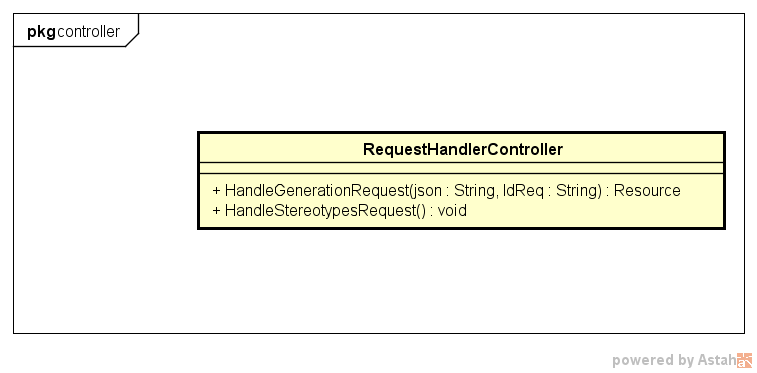
\includegraphics[width=1\textwidth]{img/server_controller}}
	\caption{Diagramma package server::controller}
\end{figure}
\begin{itemize}
\item \textbf{Descrizione}\\
Questo package contiene i vari controller che implementano il pattern Front Controller fornito dal framework \emph{Spring}. Ogni controller dovrebbe occuparsi di gestire una richiesta e di rispondere opportunamente ad essa, attraverso l'interfaccia REST definita.
\item \textbf{Padre}: \hyperref[\nogloxy{swedesigner::server}]{\nogloxy{\texttt{server}}}
\end{itemize}
\subsubsection{Classi}
\subsubsubsection{\nogloxy{swedesigner::server::controller::RequestHandlerController}}
\label{\nogloxy{swedesigner::server::controller::RequestHandlerController}}
\begin{itemize}
\item \textbf{Descrizione}\\
questa classe si occupa di ricevere le richieste REST provenienti dal client.
\item \textbf{Utilizzo}\\
essa deve gestire la richiesta di generazione di un progetto (attraverso file JSON) generando il codice e ritornandolo all'utente; inoltre essa deve restituire l'elenco degli stereotipi esistenti all'interno del server, con meta-attributi e meta-classi.
Richiama in ordine le varie classi addette alla generazione del codice, ovvero: un \texttt{Parser}, un \texttt{Generator}, un \texttt{Compiler} e infine il \texttt{Compressor}. 
\item \textbf{Relazioni con altre classi}:
\begin{itemize}
\item \textit{OUT} \hyperref[\nogloxy{swedesigner::server::compiler::Compiler}]{\nogloxy{\texttt{Compiler}}}\\
questa interfaccia si occupa di fornire un oggetto compiler generico a chi lo richiede in modo da poter rendere entensibile il sistema aggiungendo un'implementazione concreta del compiler del linguaggio target desiderato.
\item \textit{OUT} \hyperref[\nogloxy{swedesigner::server::generator::Generator}]{\nogloxy{\texttt{Generator}}}\\
questa interfaccia si occupa di fornire un oggetto \texttt{Generator} generico a chi lo richiede in modo da poter rendere entensibile il sistema aggiungendo un'implementazione concreta del generator del linguaggio target desiderato.
\item \textit{OUT} \hyperref[\nogloxy{swedesigner::server::parser::Parser}]{\nogloxy{\texttt{Parser}}}\\
questa classe si occupa di elaborare il file JSON proveniente dal client e di creare da esso un oggetto Java \texttt{ParsedProgram} strutturato in modo da poter essere facilmente convertito in codice.
\item \textit{OUT} \hyperref[\nogloxy{swedesigner::server::utility::Compressor}]{\nogloxy{\texttt{Compressor}}}\\
questa classe si occupa di creare e salvare su disco un archivio compresso contenente il progetto JSON, il codice sorgente e l'eseguibile generato che verrà poi messo a disposizione dell'utente che potrà scaricarlo.
\end{itemize}
\end{itemize}
\subsection{\nogloxy{swedesigner::server::generator}}
\label{\nogloxy{swedesigner::server::generator}}
\subsubsection{Informazioni generali}
\begin{figure}[H]
	\makebox[\textwidth][c]{
	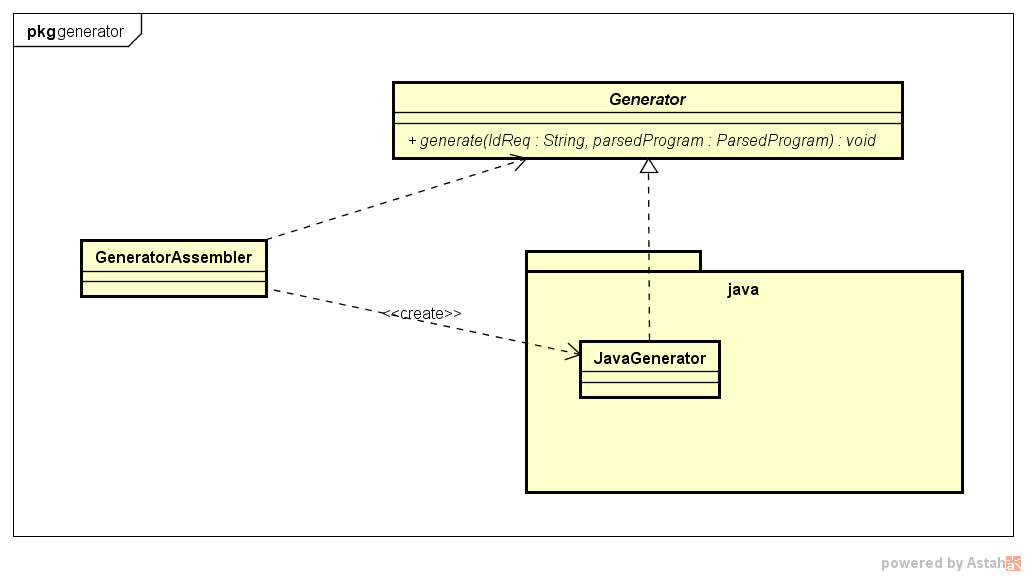
\includegraphics[width=1\textwidth]{img/server_generator}}
	\caption{Diagramma package server::generator}
\end{figure}
\begin{itemize}
\item \textbf{Descrizione}\\
Questo package contiene le classi adibite alla trasformazione dal diagramma (rappresentato in oggetti Java derivati da oggetti JSON) a codice sorgente, nel linguaggio target specifico. È stata prevista la possibilità di ampliare questo package inserendo al suo interno ulteriori package. All'interno di questo package è presente unicamente il package \texttt{java}.
\item \textbf{Padre}: \hyperref[\nogloxy{swedesigner::server}]{\nogloxy{\texttt{server}}}
\item \textbf{Package contenuti}:
\begin{itemize}
\item \hyperref[\nogloxy{swedesigner::server::generator::java}]{\nogloxy{\texttt{java}}}\\
Questo package offre un'implementazione dell'interfaccia \texttt{Generator} appartenente al package superiore. Possono essere aggiunti simili package per permettere la generazione in altri linguaggi.
\end{itemize}
\end{itemize}
\subsubsection{Classi}
\subsubsubsection{\nogloxy{swedesigner::server::generator::Generator}}
\label{\nogloxy{swedesigner::server::generator::Generator}}
\begin{itemize}
\item \textbf{Descrizione}\\
questa interfaccia si occupa di fornire un oggetto \texttt{Generator} generico a chi lo richiede in modo da poter rendere entensibile il sistema aggiungendo un'implementazione concreta del generator del linguaggio target desiderato.
\item \textbf{Utilizzo}\\
\texttt{RequestHandlerController} ha una dipendenza verso \texttt{Generator} in quanto chiederà a \texttt{GeneratorAssembler} una implementazione concreta di un \texttt{Generator} in base al linguaggio target. Il pattern realizzato con questa classe è una \emph{dependency injection}.
\item \textbf{Relazioni con altre classi}:
\begin{itemize}
\item \textit{IN} \hyperref[\nogloxy{swedesigner::server::controller::RequestHandlerController}]{\nogloxy{\texttt{RequestHandlerController}}}\\
questa classe si occupa di ricevere le richieste REST provenienti dal client.
\item \textit{IN} \hyperref[\nogloxy{swedesigner::server::generator::java::JavaGenerator}]{\nogloxy{\texttt{JavaGenerator}}}\\
questa classe è una implementazione di \texttt{Compiler} che permette di creare del codice sorgente Java da un \texttt{ParsedProgram}.
\item \textit{OUT} \hyperref[\nogloxy{swedesigner::server::project::ParsedElement}]{\nogloxy{\texttt{ParsedElement}}}\\
questa classe descrive il contratto di un elemento generico \texttt{Parsed}. Si specifica il metodo \texttt{RenderTemplate} che impone la necessità di implementarlo ad ogni classe sottostante.
\item \textit{OUT} \hyperref[\nogloxy{swedesigner::server::template::Template}]{\nogloxy{\texttt{Template}}}\\
questa interfaccia si occupa di fornire un oggetto template generico a chi lo richiede in modo da poter rendere estensibile il sistema aggiungendo un'implementazione concreta del template del linguaggio target desiderato.
\end{itemize}
\end{itemize}
\subsection{\nogloxy{swedesigner::server::generator::java}}
\label{\nogloxy{swedesigner::server::generator::java}}
\subsubsection{Informazioni generali}
\begin{itemize}
\item \textbf{Descrizione}\\
Questo package offre un'implementazione dell'interfaccia \texttt{Generator} appartenente al package superiore. Possono essere aggiunti simili package per permettere la generazione in altri linguaggi.
\item \textbf{Padre}: \hyperref[\nogloxy{swedesigner::server::generator}]{\nogloxy{\texttt{generator}}}
\end{itemize}
\subsubsection{Classi}
\subsubsubsection{\nogloxy{swedesigner::server::generator::java::JavaGenerator}}
\label{\nogloxy{swedesigner::server::generator::java::JavaGenerator}}
\begin{itemize}
\item \textbf{Descrizione}\\
questa classe è una implementazione di \texttt{Compiler} che permette di creare del codice sorgente Java da un \texttt{ParsedProgram}.
\item \textbf{Utilizzo}\\
viene utilizzata da \texttt{CompilerAssembler} che ritorna un' istanza di essa quando richiesto.
\item \textbf{Relazioni con altre classi}:
\begin{itemize}
\item \textit{OUT} \hyperref[\nogloxy{swedesigner::server::generator::Generator}]{\nogloxy{\texttt{Generator}}}\\
questa interfaccia si occupa di fornire un oggetto \texttt{Generator} generico a chi lo richiede in modo da poter rendere entensibile il sistema aggiungendo un'implementazione concreta del generator del linguaggio target desiderato.
\end{itemize}
\end{itemize}
\subsection{\nogloxy{swedesigner::server::parser}}
\label{\nogloxy{swedesigner::server::parser}}
\subsubsection{Informazioni generali}
\begin{figure}[H]
	\makebox[\textwidth][c]{
	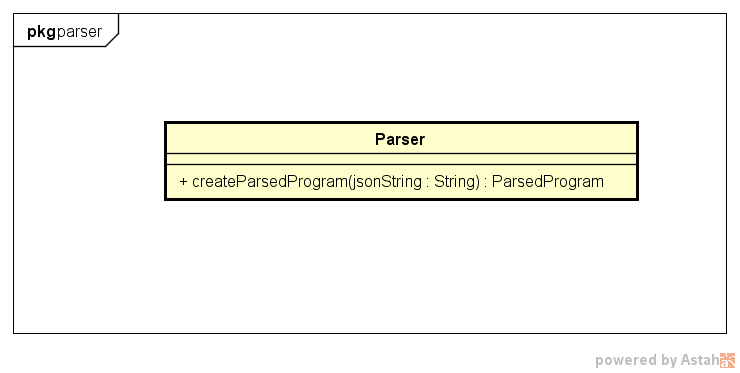
\includegraphics[width=1\textwidth]{img/server_parser}}
	\caption{Diagramma package server::parser}
\end{figure}
\begin{itemize}
\item \textbf{Descrizione}\\
Questo package presenta le classi utili all'attività di parsing dei dati ricevuti dai client.
\item \textbf{Padre}: \hyperref[\nogloxy{swedesigner::server}]{\nogloxy{\texttt{server}}}
\end{itemize}
\subsubsection{Classi}
\subsubsubsection{\nogloxy{swedesigner::server::parser::Parser}}
\label{\nogloxy{swedesigner::server::parser::Parser}}
\begin{itemize}
\item \textbf{Descrizione}\\
questa classe si occupa di elaborare il file JSON proveniente dal client e di creare da esso un oggetto Java \texttt{ParsedProgram} strutturato in modo da poter essere facilmente convertito in codice.
\item \textbf{Utilizzo}\\
viene utilizzata da \texttt{RequestHandlerController} che ne crea un istanza e ne chiama i metodi per elaborare il JSON. \texttt{Parser} inoltre crea istanze di \texttt{ParsedElement} e ritorna a controller un'istanza di \texttt{ParsedProgram}.
\item \textbf{Relazioni con altre classi}:
\begin{itemize}
\item \textit{IN} \hyperref[\nogloxy{swedesigner::server::controller::RequestHandlerController}]{\nogloxy{\texttt{RequestHandlerController}}}\\
questa classe si occupa di ricevere le richieste REST provenienti dal client.
\item \textit{OUT} \hyperref[\nogloxy{swedesigner::server::project::ParsedProgram}]{\nogloxy{\texttt{ParsedProgram}}}\\
questa classe rappresenta l'entità che possiede al suo interno tutte le componenti di un progetto. Essa possiede più \texttt{ParsedType}.
\end{itemize}
\end{itemize}
\subsection{\nogloxy{swedesigner::server::project}}
\label{\nogloxy{swedesigner::server::project}}
\subsubsection{Informazioni generali}
\begin{figure}[H]
	\makebox[\textwidth][c]{
	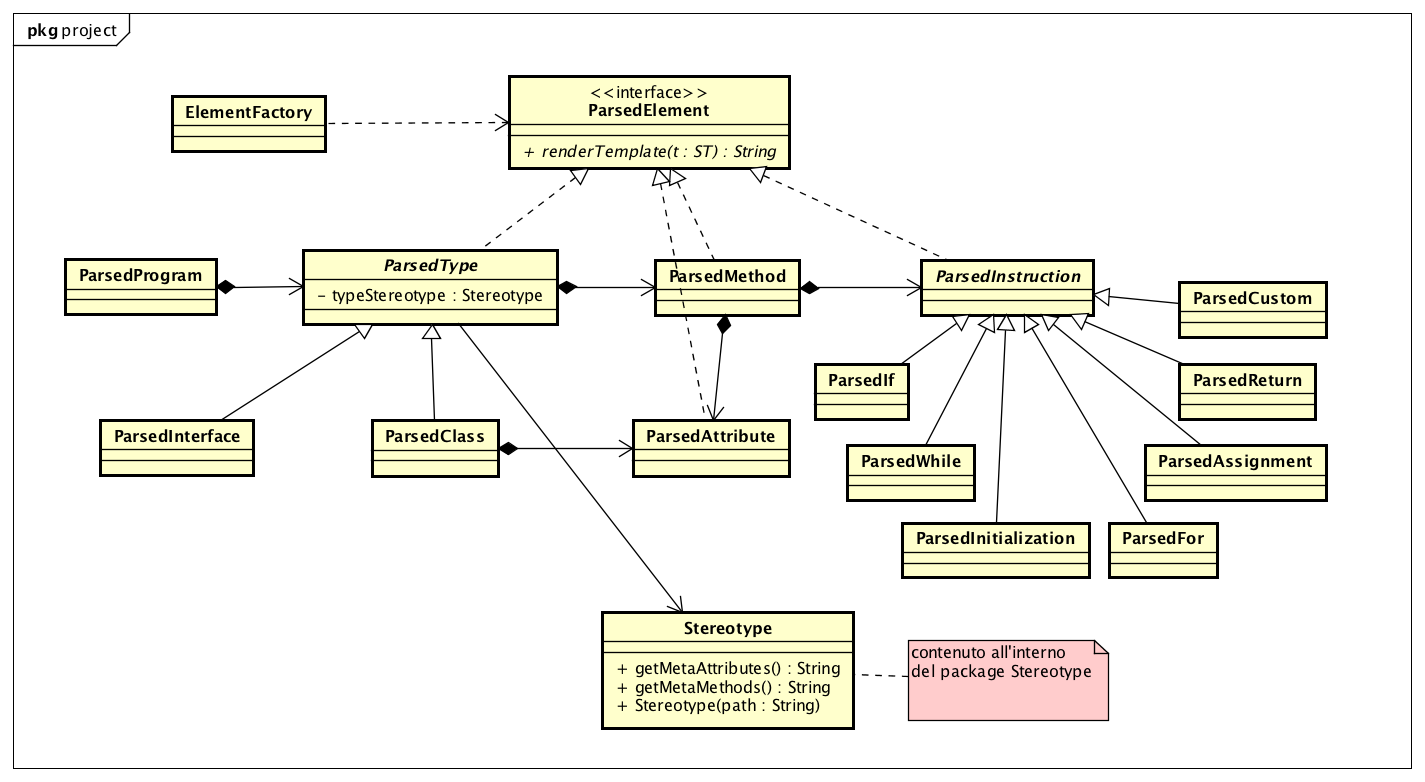
\includegraphics[width=1\textwidth]{img/server_project}}
	\caption{Diagramma package server::project}
\end{figure}
\begin{itemize}
\item \textbf{Descrizione}\\
Questo package contiene al suo interno le classi utili a rappresentare un progetto UML. Il package parser necessita di questo package per poter dare in output un programma rappresentato in memoria come oggetti Java. Per chiarezza e per evitare l'uso di keyword riservate dal linguaggio Java, all'inizio del nome di queste classi è inserito il prefisso \texttt{Parsed} (e.g. \texttt{ParsedClass}).
\item \textbf{Padre}: \hyperref[\nogloxy{swedesigner::server}]{\nogloxy{\texttt{server}}}
\end{itemize}
\subsubsection{Classi}
\subsubsubsection{\nogloxy{swedesigner::server::project::ParsedAttribute}}
\label{\nogloxy{swedesigner::server::project::ParsedAttribute}}
\begin{itemize}
\item \textbf{Descrizione}\\
questa classe rappresenta un singolo attributo, memorizzando il nome della variabile, la sua visibilità e il suo valore di default. Viene utilizzata anche per rappresentare i parametri dei metodi.
% Tuttavia, ciò non vale per attributi statici. 
% Nella \emph{Definizione_di_prodotto_v_1_0_0} [RIFERIMENTO] sarà esplicitata l'implementazione di dettaglio decisa.
\item \textbf{Utilizzo}\\
questa classe è usata da \texttt{ParsedMethod},  \texttt{ParsedClass} e \texttt{ParsedInterface} (le interfacce possono però contenere solo costanti di classe).
Questa classe implementa l'interfaccia \texttt{ParsedElement}.
Nota: Memorizzare il valore di questo attributo risulta superfluo, in quanto questo può essere impostato da un \texttt{ParsedAssignment}. 

\item \textbf{Relazioni con altre classi}:
\begin{itemize}
\item \textit{IN} \hyperref[\nogloxy{swedesigner::server::project::ParsedClass}]{\nogloxy{\texttt{ParsedClass}}}\\
questa classe estende la classe astratta \texttt{ParsedType}, imponendo al suo interno la presenza di una lista di \texttt{ParsedAttribute}. 
\item \textit{IN} \hyperref[\nogloxy{swedesigner::server::project::ParsedMethod}]{\nogloxy{\texttt{ParsedMethod}}}\\
questa classe rappresenta un metodo come insieme di istruzioni \texttt{ParsedIstruction} e un insieme di \texttt{ParsedAttribute} come parametri del metodo.
\item \textit{IN} \hyperref[\nogloxy{swedesigner::server::project::ParsedMethod}]{\nogloxy{\texttt{ParsedMethod}}}\\
questa classe rappresenta un metodo come insieme di istruzioni \texttt{ParsedIstruction} e un insieme di \texttt{ParsedAttribute} come parametri del metodo.
\item \textit{OUT} \hyperref[\nogloxy{swedesigner::server::project::ParsedElement}]{\nogloxy{\texttt{ParsedElement}}}\\
questa classe descrive il contratto di un elemento generico \texttt{Parsed}. Si specifica il metodo \texttt{RenderTemplate} che impone la necessità di implementarlo ad ogni classe sottostante.
\end{itemize}
\end{itemize}

\subsubsubsection{\nogloxy{swedesigner::server::project::ParsedClass}}
\label{\nogloxy{swedesigner::server::project::ParsedClass}}
\begin{itemize}
\item \textbf{Descrizione}\\
questa classe estende la classe astratta \texttt{ParsedType}, imponendo al suo interno la presenza di una lista di \texttt{ParsedAttribute}. 
\item \textbf{Utilizzo}\\
questa classe è creata tramite la \texttt{ElementFactory} durante il parsing del progetto e inserita all'interno di \texttt{ParsedProgram}.
\item \textbf{Classi ereditate}:
\begin{itemize}
\item \hyperref[\nogloxy{swedesigner::server::project::ParsedType}]{\nogloxy{\texttt{ParsedType}}}
\end{itemize}
\item \textbf{Relazioni con altre classi}:
\begin{itemize}
\item \textit{IN} \hyperref[\nogloxy{swedesigner::server::project::ParsedException}]{\nogloxy{\texttt{ParsedException}}}\\
Questa classe rappresenta una eccezione che viene sollevata nel momento in cui viene identificata una illegalità nel parsing della stringa in formato .json
\item \textit{OUT} \hyperref[\nogloxy{swedesigner::server::project::ParsedAttribute}]{\nogloxy{\texttt{ParsedAttribute}}}\\
questa classe rappresenta un singolo attributo, memorizzando il nome della variabile, la sua visibilità e il suo valore di default. Viene utilizzata anche per rappresentare i parametri dei metodi.
% Tuttavia, ciò non vale per attributi statici. 
% Nella \emph{Definizione_di_prodotto_v_1_0_0} [RIFERIMENTO] sarà esplicitata l'implementazione di dettaglio decisa.
\item \textit{OUT} \hyperref[\nogloxy{swedesigner::server::project::ParsedMethod}]{\nogloxy{\texttt{ParsedMethod}}}\\
questa classe rappresenta un metodo come insieme di istruzioni \texttt{ParsedIstruction} e un insieme di \texttt{ParsedAttribute} come parametri del metodo.
\end{itemize}
\end{itemize}

\subsubsubsection{\nogloxy{swedesigner::server::project::ParsedCustom}}
\label{\nogloxy{swedesigner::server::project::ParsedCustom}}
\begin{itemize}
\item \textbf{Descrizione}\\
questa classe descrive il comportamento di un blocco di codice custom, scritto nel linguaggio target.	
\item \textbf{Utilizzo}\\
dispone della possibilità di effettuare il render di un template in ingresso.
\item \textbf{Classi ereditate}:
\begin{itemize}
\item \hyperref[\nogloxy{swedesigner::server::project::ParsedInstruction}]{\nogloxy{\texttt{ParsedInstruction}}}
\end{itemize}
\end{itemize}

\subsubsubsection{\nogloxy{swedesigner::server::project::ParsedElement}}
\label{\nogloxy{swedesigner::server::project::ParsedElement}}
\begin{itemize}
\item \textbf{Descrizione}\\
questa classe descrive il contratto di un elemento generico \texttt{Parsed}. Si specifica il metodo \texttt{RenderTemplate} che impone la necessità di implementarlo ad ogni classe sottostante.
\item \textbf{Utilizzo}\\
questa interfaccia è usata da \texttt{ElementFactory}, la quale fornisce un metodo per creare nuovi elementi secondo il design pattern Factory. %[RIFERIMENTO AD APPENDICE].
\item \textbf{Sottoclassi}:
\begin{itemize}
\item \hyperref[\nogloxy{swedesigner::server::project::ParsedMethod}]{\nogloxy{\texttt{ParsedMethod}}}
\end{itemize}
\item \textbf{Relazioni con altre classi}:
\begin{itemize}
\item \textit{IN} \hyperref[\nogloxy{swedesigner::server::generator::Generator}]{\nogloxy{\texttt{Generator}}}\\
questa interfaccia si occupa di fornire un oggetto \texttt{Generator} generico a chi lo richiede in modo da poter rendere entensibile il sistema aggiungendo un'implementazione concreta del generator del linguaggio target desiderato.
\item \textit{IN} \hyperref[\nogloxy{swedesigner::server::project::ParsedAttribute}]{\nogloxy{\texttt{ParsedAttribute}}}\\
questa classe rappresenta un singolo attributo, memorizzando il nome della variabile, la sua visibilità e il suo valore di default. Viene utilizzata anche per rappresentare i parametri dei metodi.
% Tuttavia, ciò non vale per attributi statici. 
% Nella \emph{Definizione_di_prodotto_v_1_0_0} [RIFERIMENTO] sarà esplicitata l'implementazione di dettaglio decisa.
\item \textit{IN} \hyperref[\nogloxy{swedesigner::server::project::ParsedInstruction}]{\nogloxy{\texttt{ParsedInstruction}}}\\
questa classe astratta rappresenta la singola istruzione contenuta all'interno di un metodo. Essa è estesa dalle istruzioni specifiche (e.g. \texttt{ParsedIf}, \texttt{ParsedWhile}, etc.)
\item \textit{IN} \hyperref[\nogloxy{swedesigner::server::project::ParsedMethod}]{\nogloxy{\texttt{ParsedMethod}}}\\
questa classe rappresenta un metodo come insieme di istruzioni \texttt{ParsedIstruction} e un insieme di \texttt{ParsedAttribute} come parametri del metodo.
\item \textit{IN} \hyperref[\nogloxy{swedesigner::server::project::ParsedMethod}]{\nogloxy{\texttt{ParsedMethod}}}\\
questa classe rappresenta un metodo come insieme di istruzioni \texttt{ParsedIstruction} e un insieme di \texttt{ParsedAttribute} come parametri del metodo.
\item \textit{IN} \hyperref[\nogloxy{swedesigner::server::project::ParsedType}]{\nogloxy{\texttt{ParsedType}}}\\
questa classe astratta definisce un contratto comune tra le classi \texttt{ParsedInterface} e \texttt{ParsedClass}. 
\end{itemize}
\end{itemize}

\subsubsubsection{\nogloxy{swedesigner::server::project::ParsedElse}}
\label{\nogloxy{swedesigner::server::project::ParsedElse}}
\begin{itemize}
\item \textbf{Descrizione}\\
questa classe descrive il comportamento di un blocco \texttt{else}.
\item \textbf{Utilizzo}\\
dispone della possibilità di effettuare il render di un template in ingresso.
\item \textbf{Classi ereditate}:
\begin{itemize}
\item \hyperref[\nogloxy{swedesigner::server::project::ParsedInstruction}]{\nogloxy{\texttt{ParsedInstruction}}}
\end{itemize}
\end{itemize}

\subsubsubsection{\nogloxy{swedesigner::server::project::ParsedException}}
\label{\nogloxy{swedesigner::server::project::ParsedException}}
\begin{itemize}
\item \textbf{Descrizione}\\
Questa classe rappresenta una eccezione che viene sollevata nel momento in cui viene identificata una illegalità nel parsing della stringa in formato .json
\item \textbf{Utilizzo}\\
\texttt{ParsedInterface} solleva un'eccezione nel caso in cui venga identificata una illegalità nel parsing di una interfaccia. Inoltre \texttt{ParsedClass} solleva tale eccezione nel caso venga identificata una illegalità nel parsing di una classe.
\item \textbf{Relazioni con altre classi}:
\begin{itemize}
\item \textit{OUT} \hyperref[\nogloxy{swedesigner::server::project::ParsedClass}]{\nogloxy{\texttt{ParsedClass}}}\\
questa classe estende la classe astratta \texttt{ParsedType}, imponendo al suo interno la presenza di una lista di \texttt{ParsedAttribute}. 
\item \textit{OUT} \hyperref[\nogloxy{swedesigner::server::project::ParsedInterface}]{\nogloxy{\texttt{ParsedInterface}}}\\
questa classe estende la classe astratta \textt{ParsedType} ed ha bisogno soltanto della firma dei metodi essendo una classe che contiene informazioni riguardo un'interfaccia pura.
\end{itemize}
\end{itemize}

\subsubsubsection{\nogloxy{swedesigner::server::project::ParsedFor}}
\label{\nogloxy{swedesigner::server::project::ParsedFor}}
\begin{itemize}
\item \textbf{Descrizione}\\
questa classe descrive il comportamento di un blocco \texttt{for}.
\item \textbf{Utilizzo}\\
dispone della possibilità di effettuare il render di un template in ingresso.
\item \textbf{Classi ereditate}:
\begin{itemize}
\item \hyperref[\nogloxy{swedesigner::server::project::ParsedInstruction}]{\nogloxy{\texttt{ParsedInstruction}}}
\end{itemize}
\end{itemize}

\subsubsubsection{\nogloxy{swedesigner::server::project::ParsedIf}}
\label{\nogloxy{swedesigner::server::project::ParsedIf}}
\begin{itemize}
\item \textbf{Descrizione}\\
questa classe descrive il comportamento di un blocco \texttt{if}.
\item \textbf{Utilizzo}\\
dispone della possibilità di effettuare il render di un template in ingresso.
\item \textbf{Classi ereditate}:
\begin{itemize}
\item \hyperref[\nogloxy{swedesigner::server::project::ParsedInstruction}]{\nogloxy{\texttt{ParsedInstruction}}}
\end{itemize}
\end{itemize}

\subsubsubsection{\nogloxy{swedesigner::server::project::ParsedInstruction}}
\label{\nogloxy{swedesigner::server::project::ParsedInstruction}}
\begin{itemize}
\item \textbf{Descrizione}\\
questa classe astratta rappresenta la singola istruzione contenuta all'interno di un metodo. Essa è estesa dalle istruzioni specifiche (e.g. \texttt{ParsedIf}, \texttt{ParsedWhile}, etc.)
\item \textbf{Utilizzo}\\
questa classe implementa l'interfaccia \texttt{ParsedElement}.
\item \textbf{Sottoclassi}:
\begin{itemize}
\item \hyperref[\nogloxy{swedesigner::server::project::ParsedCustom}]{\nogloxy{\texttt{ParsedCustom}}}
\item \hyperref[\nogloxy{swedesigner::server::project::ParsedElse}]{\nogloxy{\texttt{ParsedElse}}}
\item \hyperref[\nogloxy{swedesigner::server::project::ParsedFor}]{\nogloxy{\texttt{ParsedFor}}}
\item \hyperref[\nogloxy{swedesigner::server::project::ParsedIf}]{\nogloxy{\texttt{ParsedIf}}}
\item \hyperref[\nogloxy{swedesigner::server::project::ParsedReturn}]{\nogloxy{\texttt{ParsedReturn}}}
\item \hyperref[\nogloxy{swedesigner::server::project::ParsedStatement}]{\nogloxy{\texttt{ParsedStatement}}}
\item \hyperref[\nogloxy{swedesigner::server::project::ParsedWhile}]{\nogloxy{\texttt{ParsedWhile}}}
\end{itemize}
\item \textbf{Relazioni con altre classi}:
\begin{itemize}
\item \textit{IN} \hyperref[\nogloxy{swedesigner::server::project::ParsedMethod}]{\nogloxy{\texttt{ParsedMethod}}}\\
questa classe rappresenta un metodo come insieme di istruzioni \texttt{ParsedIstruction} e un insieme di \texttt{ParsedAttribute} come parametri del metodo.
\item \textit{IN} \hyperref[\nogloxy{swedesigner::server::project::ParsedMethod}]{\nogloxy{\texttt{ParsedMethod}}}\\
questa classe rappresenta un metodo come insieme di istruzioni \texttt{ParsedIstruction} e un insieme di \texttt{ParsedAttribute} come parametri del metodo.
\item \textit{OUT} \hyperref[\nogloxy{swedesigner::server::project::ParsedElement}]{\nogloxy{\texttt{ParsedElement}}}\\
questa classe descrive il contratto di un elemento generico \texttt{Parsed}. Si specifica il metodo \texttt{RenderTemplate} che impone la necessità di implementarlo ad ogni classe sottostante.
\end{itemize}
\end{itemize}

\subsubsubsection{\nogloxy{swedesigner::server::project::ParsedInterface}}
\label{\nogloxy{swedesigner::server::project::ParsedInterface}}
\begin{itemize}
\item \textbf{Descrizione}\\
questa classe estende la classe astratta \textt{ParsedType} ed ha bisogno soltanto della firma dei metodi essendo una classe che contiene informazioni riguardo un'interfaccia pura.
\item \textbf{Utilizzo}\\
questa classe è creata tramite la \texttt{ElementFactory} durante il parsing del progetto e inserita all'interno di \texttt{ParsedProgram}.
\item \textbf{Classi ereditate}:
\begin{itemize}
\item \hyperref[\nogloxy{swedesigner::server::project::ParsedType}]{\nogloxy{\texttt{ParsedType}}}
\end{itemize}
\item \textbf{Relazioni con altre classi}:
\begin{itemize}
\item \textit{IN} \hyperref[\nogloxy{swedesigner::server::project::ParsedException}]{\nogloxy{\texttt{ParsedException}}}\\
Questa classe rappresenta una eccezione che viene sollevata nel momento in cui viene identificata una illegalità nel parsing della stringa in formato .json
\item \textit{OUT} \hyperref[\nogloxy{swedesigner::server::project::ParsedMethod}]{\nogloxy{\texttt{ParsedMethod}}}\\
questa classe rappresenta un metodo come insieme di istruzioni \texttt{ParsedIstruction} e un insieme di \texttt{ParsedAttribute} come parametri del metodo.
\end{itemize}
\end{itemize}

\subsubsubsection{\nogloxy{swedesigner::server::project::ParsedMethod}}
\label{\nogloxy{swedesigner::server::project::ParsedMethod}}
\begin{itemize}
\item \textbf{Descrizione}\\
questa classe rappresenta un metodo come insieme di istruzioni \texttt{ParsedIstruction} e un insieme di \texttt{ParsedAttribute} come parametri del metodo.
\item \textbf{Utilizzo}\\
questa classe è usata da \texttt{ParsedType} come descritto in precedenza. La classe inoltre implementa l'interfaccia \texttt{ParsedElement}.
\item \textbf{Classi ereditate}:
\begin{itemize}
\item \hyperref[\nogloxy{swedesigner::server::project::ParsedElement}]{\nogloxy{\texttt{ParsedElement}}}
\end{itemize}
\item \textbf{Relazioni con altre classi}:
\begin{itemize}
\item \textit{IN} \hyperref[\nogloxy{swedesigner::server::project::ParsedClass}]{\nogloxy{\texttt{ParsedClass}}}\\
questa classe estende la classe astratta \texttt{ParsedType}, imponendo al suo interno la presenza di una lista di \texttt{ParsedAttribute}. 
\item \textit{IN} \hyperref[\nogloxy{swedesigner::server::project::ParsedInterface}]{\nogloxy{\texttt{ParsedInterface}}}\\
questa classe estende la classe astratta \textt{ParsedType} ed ha bisogno soltanto della firma dei metodi essendo una classe che contiene informazioni riguardo un'interfaccia pura.
\item \textit{IN} \hyperref[\nogloxy{swedesigner::server::project::ParsedType}]{\nogloxy{\texttt{ParsedType}}}\\
questa classe astratta definisce un contratto comune tra le classi \texttt{ParsedInterface} e \texttt{ParsedClass}. 
\item \textit{OUT} \hyperref[\nogloxy{swedesigner::server::project::ParsedAttribute}]{\nogloxy{\texttt{ParsedAttribute}}}\\
questa classe rappresenta un singolo attributo, memorizzando il nome della variabile, la sua visibilità e il suo valore di default. Viene utilizzata anche per rappresentare i parametri dei metodi.
% Tuttavia, ciò non vale per attributi statici. 
% Nella \emph{Definizione_di_prodotto_v_1_0_0} [RIFERIMENTO] sarà esplicitata l'implementazione di dettaglio decisa.
\item \textit{OUT} \hyperref[\nogloxy{swedesigner::server::project::ParsedAttribute}]{\nogloxy{\texttt{ParsedAttribute}}}\\
questa classe rappresenta un singolo attributo, memorizzando il nome della variabile, la sua visibilità e il suo valore di default. Viene utilizzata anche per rappresentare i parametri dei metodi.
% Tuttavia, ciò non vale per attributi statici. 
% Nella \emph{Definizione_di_prodotto_v_1_0_0} [RIFERIMENTO] sarà esplicitata l'implementazione di dettaglio decisa.
\item \textit{OUT} \hyperref[\nogloxy{swedesigner::server::project::ParsedElement}]{\nogloxy{\texttt{ParsedElement}}}\\
questa classe descrive il contratto di un elemento generico \texttt{Parsed}. Si specifica il metodo \texttt{RenderTemplate} che impone la necessità di implementarlo ad ogni classe sottostante.
\item \textit{OUT} \hyperref[\nogloxy{swedesigner::server::project::ParsedElement}]{\nogloxy{\texttt{ParsedElement}}}\\
questa classe descrive il contratto di un elemento generico \texttt{Parsed}. Si specifica il metodo \texttt{RenderTemplate} che impone la necessità di implementarlo ad ogni classe sottostante.
\item \textit{OUT} \hyperref[\nogloxy{swedesigner::server::project::ParsedInstruction}]{\nogloxy{\texttt{ParsedInstruction}}}\\
questa classe astratta rappresenta la singola istruzione contenuta all'interno di un metodo. Essa è estesa dalle istruzioni specifiche (e.g. \texttt{ParsedIf}, \texttt{ParsedWhile}, etc.)
\item \textit{OUT} \hyperref[\nogloxy{swedesigner::server::project::ParsedInstruction}]{\nogloxy{\texttt{ParsedInstruction}}}\\
questa classe astratta rappresenta la singola istruzione contenuta all'interno di un metodo. Essa è estesa dalle istruzioni specifiche (e.g. \texttt{ParsedIf}, \texttt{ParsedWhile}, etc.)
\end{itemize}
\end{itemize}

\subsubsubsection{\nogloxy{swedesigner::server::project::ParsedProgram}}
\label{\nogloxy{swedesigner::server::project::ParsedProgram}}
\begin{itemize}
\item \textbf{Descrizione}\\
questa classe rappresenta l'entità che possiede al suo interno tutte le componenti di un progetto. Essa possiede più \texttt{ParsedType}.
\item \textbf{Utilizzo}\\
La classe \texttt{Parser} ha una dipendenza verso questo elemento: essa infatti ne crea una e la ritorna al controller, il quale la passerà alla classe \texttt{Generator}.
\item \textbf{Relazioni con altre classi}:
\begin{itemize}
\item \textit{IN} \hyperref[\nogloxy{swedesigner::server::parser::Parser}]{\nogloxy{\texttt{Parser}}}\\
questa classe si occupa di elaborare il file JSON proveniente dal client e di creare da esso un oggetto Java \texttt{ParsedProgram} strutturato in modo da poter essere facilmente convertito in codice.
\item \textit{OUT} \hyperref[\nogloxy{swedesigner::server::project::ParsedType}]{\nogloxy{\texttt{ParsedType}}}\\
questa classe astratta definisce un contratto comune tra le classi \texttt{ParsedInterface} e \texttt{ParsedClass}. 
\end{itemize}
\end{itemize}

\subsubsubsection{\nogloxy{swedesigner::server::project::ParsedReturn}}
\label{\nogloxy{swedesigner::server::project::ParsedReturn}}
\begin{itemize}
\item \textbf{Descrizione}\\
questa classe descrive il comportamento di un blocco di ritorno di un metodo.
\item \textbf{Utilizzo}\\
dispone della possibilità di effettuare il render di un template in ingresso.
\item \textbf{Classi ereditate}:
\begin{itemize}
\item \hyperref[\nogloxy{swedesigner::server::project::ParsedInstruction}]{\nogloxy{\texttt{ParsedInstruction}}}
\end{itemize}
\end{itemize}

\subsubsubsection{\nogloxy{swedesigner::server::project::ParsedStatement}}
\label{\nogloxy{swedesigner::server::project::ParsedStatement}}
\begin{itemize}
\item \textbf{Descrizione}\\
questa classe descrive il comportamento di un blocco di assegnazione variabile o inizializzazione variabile.	
\item \textbf{Utilizzo}\\
dispone della possibilità di effettuare il render di un template in ingresso.
\item \textbf{Classi ereditate}:
\begin{itemize}
\item \hyperref[\nogloxy{swedesigner::server::project::ParsedInstruction}]{\nogloxy{\texttt{ParsedInstruction}}}
\end{itemize}
\end{itemize}

\subsubsubsection{\nogloxy{swedesigner::server::project::ParsedType}}
\label{\nogloxy{swedesigner::server::project::ParsedType}}
\begin{itemize}
\item \textbf{Descrizione}\\
questa classe astratta definisce un contratto comune tra le classi \texttt{ParsedInterface} e \texttt{ParsedClass}. 
\item \textbf{Utilizzo}\\
essa possiede un insieme di \texttt{ParsedMethod}. Nell'accezione di molti linguaggi, classi e interfacce rappresentano dei tipi. Questa classe deriva da \texttt{ParsedElement} al fine di poter usare polimorfismo sugli elementi creati dal \texttt{Parser}. 
I tipi sono creati dalla \texttt{ParsedFactory} e sono richiesti da \texttt{Parser}.
\item \textbf{Sottoclassi}:
\begin{itemize}
\item \hyperref[\nogloxy{swedesigner::server::project::ParsedClass}]{\nogloxy{\texttt{ParsedClass}}}
\item \hyperref[\nogloxy{swedesigner::server::project::ParsedInterface}]{\nogloxy{\texttt{ParsedInterface}}}
\end{itemize}
\item \textbf{Relazioni con altre classi}:
\begin{itemize}
\item \textit{IN} \hyperref[\nogloxy{swedesigner::server::project::ParsedProgram}]{\nogloxy{\texttt{ParsedProgram}}}\\
questa classe rappresenta l'entità che possiede al suo interno tutte le componenti di un progetto. Essa possiede più \texttt{ParsedType}.
\item \textit{OUT} \hyperref[\nogloxy{swedesigner::server::project::ParsedElement}]{\nogloxy{\texttt{ParsedElement}}}\\
questa classe descrive il contratto di un elemento generico \texttt{Parsed}. Si specifica il metodo \texttt{RenderTemplate} che impone la necessità di implementarlo ad ogni classe sottostante.
\item \textit{OUT} \hyperref[\nogloxy{swedesigner::server::project::ParsedMethod}]{\nogloxy{\texttt{ParsedMethod}}}\\
questa classe rappresenta un metodo come insieme di istruzioni \texttt{ParsedIstruction} e un insieme di \texttt{ParsedAttribute} come parametri del metodo.
\end{itemize}
\end{itemize}

\subsubsubsection{\nogloxy{swedesigner::server::project::ParsedWhile}}
\label{\nogloxy{swedesigner::server::project::ParsedWhile}}
\begin{itemize}
\item \textbf{Descrizione}\\
questa classe descrive il comportamento di un blocco \texttt{while} e dispone della possibilità di effettuare il render di un template in ingresso.
\item \textbf{Utilizzo}\\
deriva da \texttt{ParsedInstruction}.
\item \textbf{Classi ereditate}:
\begin{itemize}
\item \hyperref[\nogloxy{swedesigner::server::project::ParsedInstruction}]{\nogloxy{\texttt{ParsedInstruction}}}
\end{itemize}
\end{itemize}
\subsection{\nogloxy{swedesigner::server::stereotype}}
\label{\nogloxy{swedesigner::server::stereotype}}
\subsubsection{Informazioni generali}
\begin{figure}[H]
	\makebox[\textwidth][c]{
	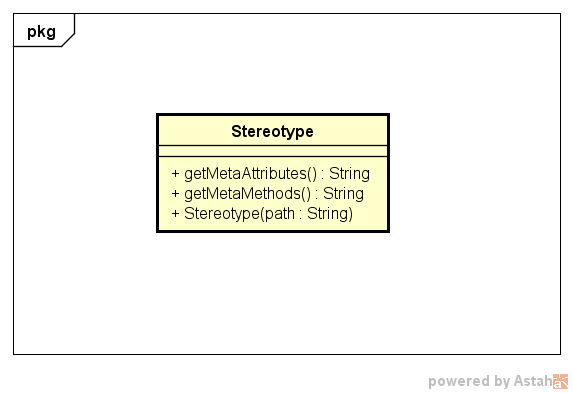
\includegraphics[width=1\textwidth]{img/server_stereotype}}
	\caption{Diagramma package server::stereotype}
\end{figure}
\begin{itemize}
\item \textbf{Descrizione}\\
Questo package offre le classi che descrivono ciò che caratterizza un particolare stereotipo. Queste classi derivano tutte da una classe base chiamata \texttt{Stereotype}. Le classi che definiscono come deve variare ogni stereotipo sono contraddistinte dal suffisso \texttt{Stereotype} (e.g. \texttt{BoardStereotype}). Si noti che tra queste classi non sono presenti dei legami, in quanto sono necessarie alla generazione del codice. La struttura degli stereotipi assegnabili ad ogni classe e le loro relazioni saranno definite successivamente nella \emph{Definizione di Prodotto}.
\item \textbf{Padre}: \hyperref[\nogloxy{swedesigner::server}]{\nogloxy{\texttt{server}}}
\end{itemize}

\subsection{\nogloxy{swedesigner::server::template}}
\label{\nogloxy{swedesigner::server::template}}
\subsubsection{Informazioni generali}
\begin{figure}[H]
	\makebox[\textwidth][c]{
	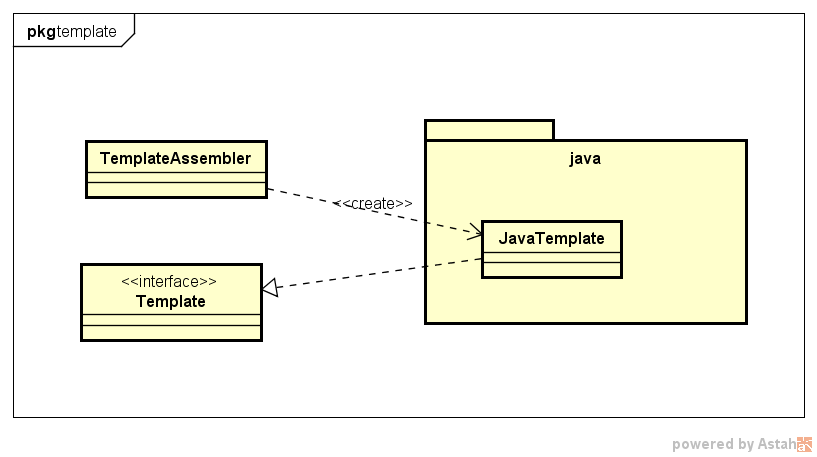
\includegraphics[width=1\textwidth]{img/server_template}}
	\caption{Diagramma package server::template}
\end{figure}
\begin{itemize}
\item \textbf{Descrizione}\\
Questo package contiene le classi necessarie a trasformare l'oggetto che rappresenta il programma in una stringa di testo che rappresenta il codice sorgente tramite un sistema a template, il quale definirà tramite dei file di testo la struttura di ogni componente del programma; per facilitare questo compito sarà usata la libreria \stringtemplate{}. Similarmente al package \texttt{Generator} si è prevista la possibilità di implementare un sistema di template per ogni linguaggio, implementando diversamente l'interfaccia della classe Template e definendo un nuovo package (e.g. \texttt{Java}).
\item \textbf{Padre}: \hyperref[\nogloxy{swedesigner::server}]{\nogloxy{\texttt{server}}}
\item \textbf{Package contenuti}:
\begin{itemize}
\item \hyperref[\nogloxy{swedesigner::server::template::java}]{\nogloxy{\texttt{java}}}\\
Questo package definisce le operazioni necessarie all'applicazione del template relativo al linguaggio Java. Simili package possono essere creati per permettere l'esportazione in diversi linguaggi target.
\end{itemize}
\end{itemize}
\subsubsection{Classi}
\subsubsubsection{\nogloxy{swedesigner::server::template::Template}}
\label{\nogloxy{swedesigner::server::template::Template}}
\begin{itemize}
\item \textbf{Descrizione}\\
questa interfaccia si occupa di fornire un oggetto template generico a chi lo richiede in modo da poter rendere estensibile il sistema aggiungendo un'implementazione concreta del template del linguaggio target desiderato.
\item \textbf{Utilizzo}\\
\texttt{RequestHandlerController} ha una dipendenza verso Template in quanto chiederà a \texttt{TemplateAssembler} una implementazione concreta di un \texttt{Template} in base al linguaggio target. Il pattern realizzato con questa classe è una \emph{dependency injection}.
\item \textbf{Relazioni con altre classi}:
\begin{itemize}
\item \textit{IN} \hyperref[\nogloxy{swedesigner::server::generator::Generator}]{\nogloxy{\texttt{Generator}}}\\
questa interfaccia si occupa di fornire un oggetto \texttt{Generator} generico a chi lo richiede in modo da poter rendere entensibile il sistema aggiungendo un'implementazione concreta del generator del linguaggio target desiderato.
\item \textit{IN} \hyperref[\nogloxy{swedesigner::server::template::java::JavaTemplate}]{\nogloxy{\texttt{JavaTemplate}}}\\
questa classe è una implementazione di \texttt{Template} che permette di fornire un template di una classe, metodo o costrutto Java.
\end{itemize}
\end{itemize}
\subsection{\nogloxy{swedesigner::server::template::java}}
\label{\nogloxy{swedesigner::server::template::java}}
\subsubsection{Informazioni generali}
\begin{itemize}
\item \textbf{Descrizione}\\
Questo package definisce le operazioni necessarie all'applicazione del template relativo al linguaggio Java. Simili package possono essere creati per permettere l'esportazione in diversi linguaggi target.
\item \textbf{Padre}: \hyperref[\nogloxy{swedesigner::server::template}]{\nogloxy{\texttt{template}}}
\end{itemize}
\subsubsection{Classi}
\subsubsubsection{\nogloxy{swedesigner::server::template::java::JavaTemplate}}
\label{\nogloxy{swedesigner::server::template::java::JavaTemplate}}
\begin{itemize}
\item \textbf{Descrizione}\\
questa classe è una implementazione di \texttt{Template} che permette di fornire un template di una classe, metodo o costrutto Java.
\item \textbf{Utilizzo}\\
viene utilizzata da \texttt{CompilerAssembler} che ritorna un' istanza di essa quando richiesto.
\item \textbf{Relazioni con altre classi}:
\begin{itemize}
\item \textit{OUT} \hyperref[\nogloxy{swedesigner::server::template::Template}]{\nogloxy{\texttt{Template}}}\\
questa interfaccia si occupa di fornire un oggetto template generico a chi lo richiede in modo da poter rendere estensibile il sistema aggiungendo un'implementazione concreta del template del linguaggio target desiderato.
\end{itemize}
\end{itemize}
\subsection{\nogloxy{swedesigner::server::utility}}
\label{\nogloxy{swedesigner::server::utility}}
\subsubsection{Informazioni generali}
\begin{figure}[H]
	\makebox[\textwidth][c]{
	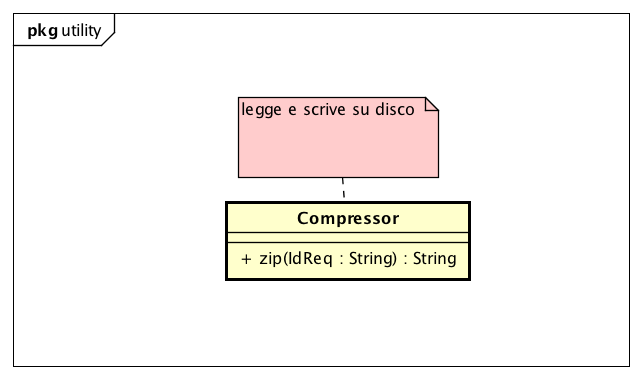
\includegraphics[width=1\textwidth]{img/server_utility}}
	\caption{Diagramma package server::utility}
\end{figure}
\begin{itemize}
\item \textbf{Descrizione}\\
Questo package contiene le componenti secondarie necessarie al server, indipendentemente dal linguaggio target dell'applicazione.
\item \textbf{Padre}: \hyperref[\nogloxy{swedesigner::server}]{\nogloxy{\texttt{server}}}
\end{itemize}
\subsubsection{Classi}
\subsubsubsection{\nogloxy{swedesigner::server::utility::Compressor}}
\label{\nogloxy{swedesigner::server::utility::Compressor}}
\begin{itemize}
\item \textbf{Descrizione}\\
questa classe si occupa di creare e salvare su disco un archivio compresso contenente il progetto JSON, il codice sorgente e l'eseguibile generato che verrà poi messo a disposizione dell'utente che potrà scaricarlo.
\item \textbf{Utilizzo}\\
viene utilizzata da \texttt{RequestHandlerController} per creare l'archivio compresso dei file
\item \textbf{Relazioni con altre classi}:
\begin{itemize}
\item \textit{IN} \hyperref[\nogloxy{swedesigner::server::controller::RequestHandlerController}]{\nogloxy{\texttt{RequestHandlerController}}}\\
questa classe si occupa di ricevere le richieste REST provenienti dal client.
\end{itemize}
\end{itemize}

\begin{adjustwidth}{-3cm}{-3cm}
	\begin{figure}[H]
		\makebox[\textwidth][c]{
		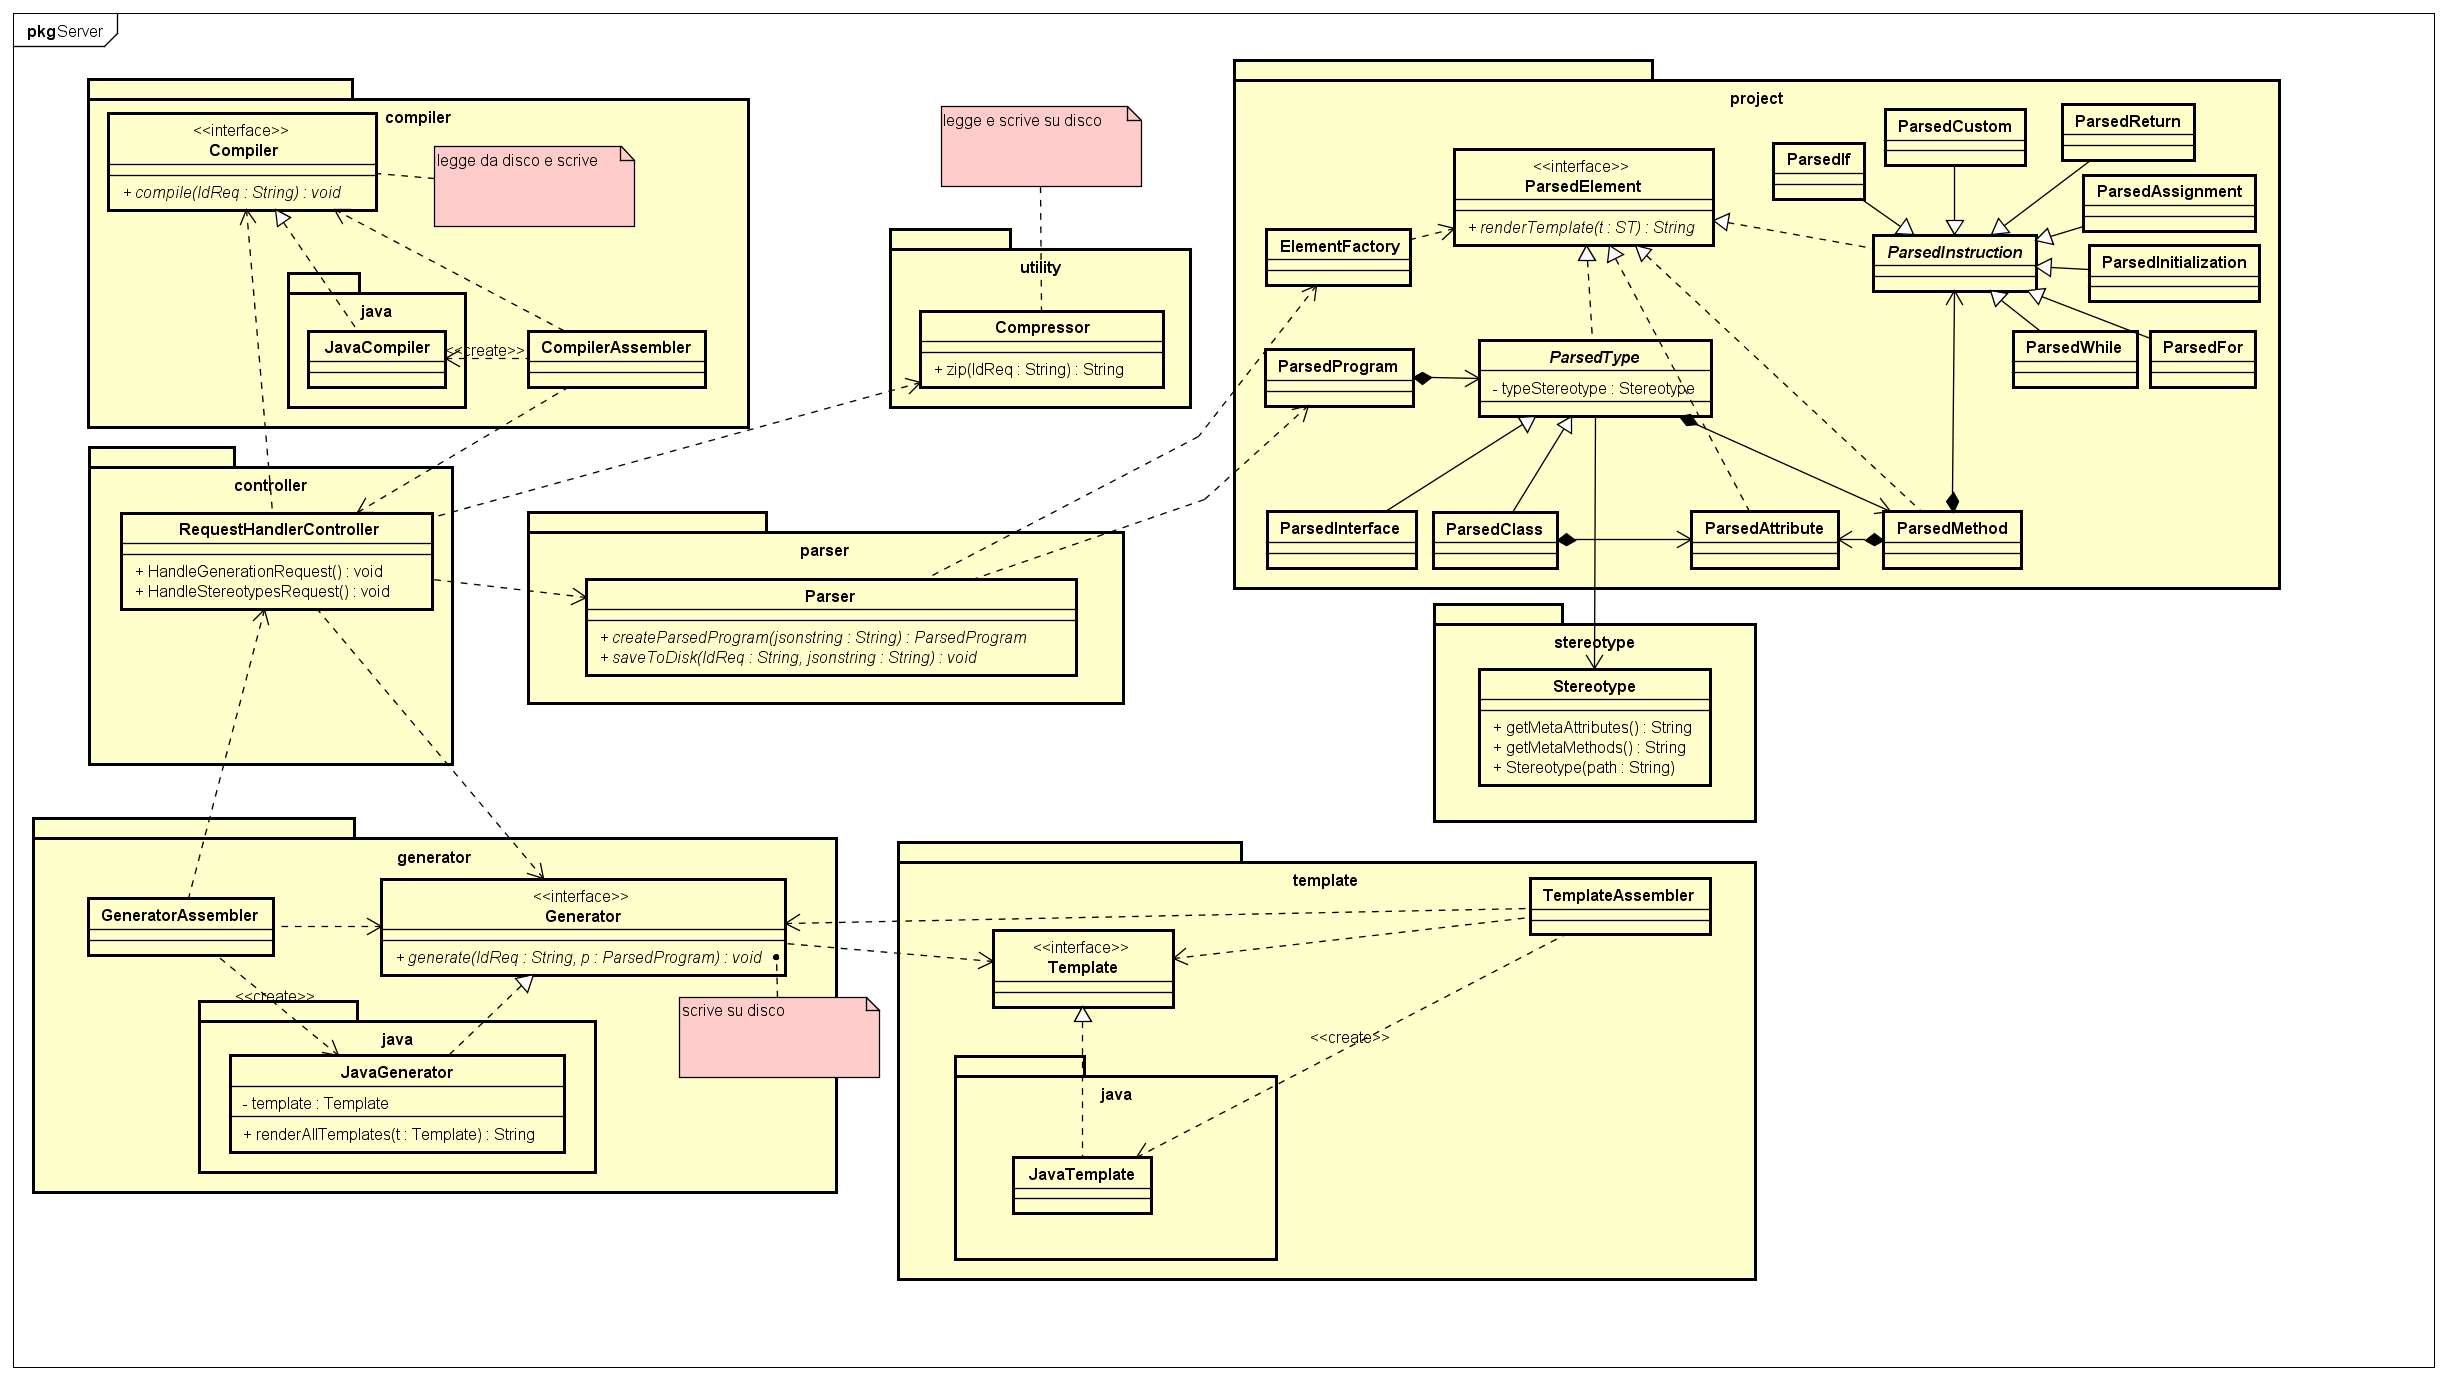
\includegraphics[width=0.9\textwidth]{img/server_pkg2}}
		\caption{Diagramma package server}
	\end{figure}
\end{adjustwidth}
